\documentclass[a4paper]{article}

\usepackage{fullpage} % Package to use full page
\usepackage{parskip} % Package to tweak paragraph skipping
\usepackage{tikz} % Package for drawing
\usepackage{amsmath}
\usepackage{hyperref}
\usepackage{flexisym}

\usepackage[a4paper]{geometry}
\usepackage{amsmath}
\usepackage{amssymb}
\usepackage{amsfonts}
%\usepackage{algorithm}
\usepackage{algorithmic}
\usepackage[]{algorithm2e}
\usepackage{graphicx}
\usepackage{color}
\usepackage[bf,SL,BF]{subfigure}
\usepackage{url}
\usepackage{pdfsync}
\usepackage[affil-it]{authblk}
\usepackage{blindtext}

\usepackage{subeqnarray}
\usepackage{cases}

\makeatletter
\@addtoreset{equation}{section}
\makeatother
\renewcommand{\theequation}{\arabic{section}.\arabic{equation}}

\usepackage{verbatim}

\title{Note about Julia Code}
\author{Haolei Wang}

\begin{document}

\maketitle
%\begin{comment}
\section{Introduction}

In this note, I will try to introduce how I write this Julia code to calculate the energy in a granular system as soon as possible. This code was based on Ortner's \texttt{\textprime JuLIP\textprime} package.

We will compare the performance of this code with my own Matlab code. It is known that Matlab deals the vector manipulation pretty well while loop rather bad. Julia can deal with loop rather well. In our project, it is rather common to use loop, so it is better to design a Julia code. 

\section{Problem Setting}
In this section, we will introduce our problem. We need to calculate the inner potential energy of a granular system. The system is a square (2D) with {\color{red}periodic boundary condition}, which is filled with two kind of disks. The number of particle of each are the same, while their radius ratio is 1.4. Particles will interact with each other only when they overlap. We give the following energy model.

\begin{equation} \label{eq: pair potential}
E_{ij} = \left\{
    \begin{aligned}
           & k\frac{(r_i+r_j - \left|\vec{x}_i-\vec{x}_j\right|)^{\alpha}}{\alpha} &  &\text{for} \quad \left|\vec{x}_i-\vec{x}_j\right|< r_i+r_j, \\
           & 0 &  &\text{for} \quad \left|\vec{x}_i-\vec{x}_j\right|\ge r_i+r_j, ,
    \end{aligned}  
\right.   i\ne j
\end{equation}
where $k$ represents the particle stiffness, $r_i$ and $r_j$ are the radii of particle $i$ and $j$ and $\vec{x}_i$ and $\vec{x}_j$ are the positions of the their centers. With different $\alpha$, we can get different kinds of pair potentials. Thus the total potential energy of the system is:
\begin{equation}\label{eq: total potential1}
     E_{total} = \sum_{i<j}E_{ij}.
\end{equation}

Since the particles only interact with each other unless they contact, we can rewrite the potential energy for a single contact $c$ as:
\begin{equation}
E_c = k\frac{\delta_c^{\alpha}}{\alpha},
\end{equation}
where $\delta_c$ is the overlap associated with the contact $c$ and according to equation \eqref{eq: pair potential}:
\begin{equation}\label{eq: overlap}
\delta_c = r_i + r_j - \left|\vec{x}_i-\vec{x}_j\right|.
\end{equation}

Thus, the total potential energy of the system is:
\begin{equation}\label{eq: total potential2}
     E_{total} = \sum_{c}E_{c}.
\end{equation}

\begin{figure}[!htbp]
\begin{center}
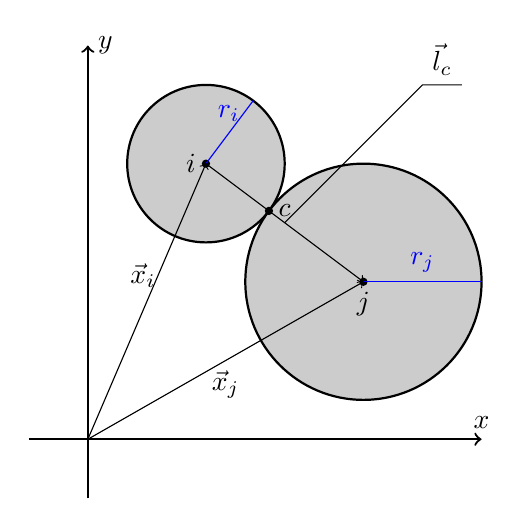
\begin{tikzpicture}
\draw [black,thick,fill=black!20] (1.5,3.5) circle (1cm) node[left] {$i$};
\fill [black] (1.5,3.5) circle (1.5pt);
\draw [blue,-] (1.5,3.5) -- (2.1,4.3) node[above] at (1.79,3.91) {$r_{i}$}; 
\draw [black,thick,fill=black!20] (3.5,2) circle (1.5cm) node[below] {$j$};
\fill [black] (3.5,2) circle (1.5pt);
\fill [black] (2.3,2.9) circle (1.5pt) node[right] {$c$};
\draw [blue,-] (3.5,2) -- (5,2) node[above] at (4.25,2) {$r_j$};
\draw [thick, ->] (-0.75,0) -- (5,0) node[above] {$x$};
\draw [thick, ->] (0,-0.75) -- (0,5) node[right] {$y$};
\draw [black,->] (0,0) -- (1.5,3.5) node[above] at (0.7,1.8) {$\vec{x}_{i}$}; 
\draw [black,->] (0,0) -- (3.5,2) node[below] at (1.75,1) {$\vec{x}_{j}$};
\draw [black,->] (1.5,3.5) -- (3.5,2);
\path[draw] (2.5,2.75) -- (4.25,4.5) -- (4.75,4.5);
\node [above] at (4.5,4.5) {$\vec{l}_c$};
\end{tikzpicture}
\end{center}
\caption{Two particles contact}
\end{figure}

\section{Programming}
In this section, we will introduce the programming approach.
\subsection{Calculating the distance between two points in periodic cell}
From section 2, we can calculate the total potential energy by summing the potential energy of all contacting particles. Thus, we need to find all the contacts. From equation \eqref{eq: overlap}, it's the key to calculate the distance of all particles with each other.

If the cell is not periodic, it's easy to calculate the distance between particles, which is the 2-norm of $\left|\vec{x}_{j}-\vec{x}_{i}\right|$. However, in our project, the cell is periodic, so we need to reconsider this when the particles are near the boundaries. Since we don't consider long-range interaction, so the distance between two points in periodic cell is the smallest of the distance of their periodic projections with each other.

Firstly, we will try to calculate the periodic distance in a unit square. In Figure 2, we have two points $i$ and $j$, with their coordination $X_i$ and $X_j$ respectively. If we set
\begin{equation}\label{eq: unit point difference1}
d\bar{X} = X_{j}-X_{i}=(d\bar{X}_{1},d\bar{X}_{2}), 
\end{equation}
we know that $-1<d\bar{X}_{k}<1, k=1,2$. For a periodic unit square, it is important to note that the real difference of two points' coordination 
$$
dX=(dX_{1},dX_{2})
$$ 
should satisfy the following condition:
$$
\left|dX_{k}\right|\le\frac{1}{2}.
$$
The relationship between $dX_{k}$ and $d\bar{X}_{k}$ is:
\begin{equation}\label{eq: unit point difference2}
dX_{k} = \text{mod}(d\bar{X}_{k} + \frac{1}{2}, 1) - \frac{1}{2}.
\end{equation}

The distance between points $i$ and $j$ is:
\begin{equation}
d_{ij}=\sqrt{dX \cdot dX}
\end{equation}

\begin{figure}[!htbp]
\begin{center}
\begin{tikzpicture}
\draw [thick, ->] (-2,0) -- (5.5,0) node[above] {$x$};
\draw [thick, ->] (0,-1) -- (0,5.5) node[right] {$y$};
\draw [thick,-] (4,0) -- (4,4) node[above] at (4.1,0) {1};
\draw [thick,-] (0,4) -- (4,4) node[left] at (0,4.1) {1};
\fill [black] (0.5,0.5) circle (1.5pt) node[right] {$i$};
\fill [black] (3,3.5) circle (1.5pt) node[right] {$j$};
\fill [black] (-1,-0.5) circle (1.5pt) node[right] {$j\textprime$};
\end{tikzpicture}
\end{center}
\caption{Points in periodic unit square}
\end{figure}

Secondly, we will consider a common deformed (simple shear) cell with periodic boundary condition. In Figure 3, the cell can be denoted using a matrix:
$$
M=
\begin{bmatrix}
L & Le\\
0 & H
\end{bmatrix}
$$
The points $i$ and $j$ in this cell can be projected in the unit square reference cell using
\begin{subequations}\label{eq: tranform x2X}
\begin{align}
\hat{X}&=M^{-1}x \\
X&=\hat{X} - \text{floor}(\hat{X})
\end{align}
\end{subequations}
where $X$ and $x$ are the coordination in the reference cell and real cell respectively. 

We can calculate the difference between two reference point, $dX$, using equation \eqref{eq: unit point difference1} and \eqref{eq: unit point difference2}. Then we can calculate the real coordination difference using
\begin{equation}\label{eq: points difference}
dx=MdX
\end{equation}

The distance between points $i$ and $j$ can be calculated by
\begin{equation}
d_{ij}=\sqrt{dx \cdot dx}
\end{equation}

\begin{figure}[!htbp]
\begin{center}
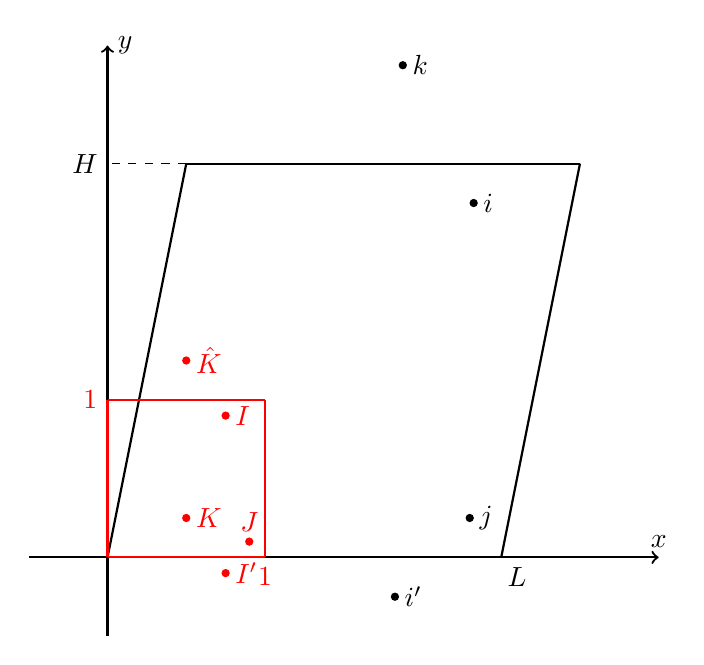
\begin{tikzpicture}
\draw [thick, ->] (-1,0) -- (7,0) node[above] {$x$};
\draw [thick, ->] (0,-1) -- (0,6.5) node[right] {$y$};
\draw [thick,-] (5,0) -- (6,5) node[below] at (5.2,0) {$L$};
\draw [thick,-] (6,5) -- (1,5);
\draw [dashed] (1,5) -- (0,5) node[left] at (0,5) {$H$};
\draw [thick,-] (1,5) -- (0,0);
\draw [red,thick,-] (2,0) -- (2,2) node[below] at (2,0) {1};
\draw [red,thick,-] (0,2) -- (2,2) node[left] at (0,2) {1};
\draw [red,thick,-] (0,0) -- (0,2); \draw [red,thick,-] (0,0) -- (2,0);
\fill [black] (4.65,4.5) circle (1.5pt) node[right] {$i$};
\fill [black] (4.6,0.5) circle (1.5pt) node[right] {$j$};
\fill [black] (3.65,-0.5) circle (1.5pt) node[right] {$i\textprime$};
\fill [red] (1.5,1.8) circle (1.5pt) node[right] {$I$};
\fill [red] (1.8,0.2) circle (1.5pt) node[above] {$J$};
\fill [red] (1.5,-0.2) circle (1.5pt) node[right] {$I\textprime$};
\fill [black] (3.75,6.25) circle (1.5pt) node[right] {$k$};
%\fill [black] (2.75,1.25) circle (1.5pt) node[right] {$\hat{k}$};
\fill [red] (1,2.5) circle (1.5pt) node[right] {$\hat{K}$};
\fill [red] (1,0.5) circle (1.5pt) node[right] {$K$};
\end{tikzpicture}
\end{center}
\caption{Points in deformed cell}
\end{figure}

\subsection{Calculate neighbourlist of granular system}
Now we know how to calculate the distance between points in periodic cell, it's identical to calculate the distance between the centers of two particles. Thus, we can determine whether two particles overlap. 

Noting that the particles interact with each other only when they overlap, we can firstly find the neighbourlist of the system. The neighbourlist stores the pairs of indexes of every two possibly overlapping particles. Thus when we calculate the total potential energy, we only need to compute the potential energy in the neighbourlist and then sum up.

Ortner provide a package called \texttt{\textprime NeighbourLists\textprime } using Julia language, which is rather fast to determine the neighbourlist based on a cutoff $r_{cut}$. Matlab also provides several functions to calculate the distance and knn (k-nearest neighbour), the relative functions are \texttt{pdist, knnsearch, rangesearch}, etc. However, the Matlab functions cannot compute the periodic distance either, so the above functions are not suitable for our project. I programmed a Matlab code to calculate periodic distance, but it couldn't manipulate large system because the space complexity is $O(N^2)$. While Ortner's code is efficient and {\color{red}with $O(N)$ space complexity (not sure if this is correct)}, this can be a big advantage. 

Package \texttt{\textprime NeighbourLists\textprime } computes the distance between particles and then determine whether the distance is smaller than $r_{cut}$. 
This package can provide the following information:
\texttt{nlist.i, nlist.j, nlist.r, nlist.R}, here \texttt{nlist} means neighbourlist, \texttt{nlist.i} and \texttt{nlist.j} are two vectors of particles' index, \texttt{nlist.r} is a vector storing distance between particles, \texttt{nlist.R} is a vector that stores $dx$ in equation \eqref{eq: points difference}. Meanwhile, \texttt{nlist.r[k]} is the distance between particle \texttt{nlist.i[k]} and \texttt{nlist.j[k]}, \texttt{nlist.R[k]} is $dx$ associated with particle \texttt{nlist.i[k]} and \texttt{nlist.j[k]}.

Even though package \texttt{\textprime NeighbourLists\textprime } is very efficient, we still find it is a waste to calculate the total neighbourlist every time when we calculate the energy, since the displacement of particles in our system is so small that the neighbourlist is almost unchanged. We only need to update \texttt{nlist.r} and \texttt{nlist.R}. If the maximum displacement reaches a tolerance $r_{tol}$, we will update the total neighbourlist.

Next, we will give the pseudocode.

\begin{verbatim}
function energy(Config, V)
    """
    Function to calculate the total potential energy.
    V(r) is the pair potential.
    """
    nlist_i, nlist_j = update_neighbourlist(Config)
    E = 0.0
    for k = 1:length(nlist_i)
        i, j = nlist_i[k], nlist_j[k];
        xi, xj = Config.X[i], Config.X[j];
        dx = xj - xi;
        dX = inv_bins * dx;                   # using equation (3.4a)
        dX = dX - floor(dX);                  # using equation (3.4b)
        dX = mod(dx + 0.5, 1) - 0.5;          # using equation (3.2)
        dx = bins * dX;                       # using equation (3.5)
        r = norm2(dx);
        E = E + V(r);
    end
    return 0.5*E
end

function update_neighbourlist(Config)
   """
   Function to update the neighbourlist
   has_data(Config, fieldname) judges if the Config structure has this field.
   """
   if has_data(Config, nlist_X)
      X_Old = Config.nlist_X;
      max_displacement = max(norm2.(Config.X - X_Old));
      if max_displacement < r_tol
          return Config.nlist_i, Config.nlist_j;
      end
   end
   nlist = NeighbourList(Config, rcut);
   Config.nlist_X, Config.nlist_i, Config.nlist_j = Config.X, nlist.i, nlist.j;
   return nlist.i, nlist.j;
end
   
\end{verbatim}

One should note that we compute $dX$ using $dx$ instead of $X$ using $x$ in the \texttt{energy} function. We will now show this.

In the pseudocode,
$$
\begin{aligned}
&X_{i} = (\varepsilon_{i}, \eta_{i})^{T}, \quad X_{j} = (\varepsilon_{j}, \eta_{j})^{T} ,\quad \text{where} \quad 0 \le \varepsilon, \eta < 1\\
 \Longrightarrow &\hat{X}_{i} = (m_{i}+\varepsilon_{i}, n_{i}+\eta_{i})^{T},\quad \hat{X}_{j} = (m_{j}+\varepsilon_{j}, n_{j}+\eta_{j})^{T},\quad \text{where} \quad m,n \in \mathbb{Z}\\
\Longrightarrow &x_{i}=M\hat{X}_{i}, \quad x_{j}=M\hat{X}_{j}\\
\Longrightarrow &dx = x_{j}-x_{i}=M(\hat{X}_{j}-\hat{X}_{i})\\
\Longrightarrow &d\hat{X} = M^{-1}dx=\hat{X}_{j}-\hat{X}_{i}=(m_{j}-m_{i}+\varepsilon_{j}-\varepsilon_{i}, n_{j}-n_{i}+\eta_{j}-\eta_{i})^{T}\\
\Longrightarrow &d\bar{X}=d\hat{X}-\text{floor}(d\hat{X})=\boxed{\text{mod}(\varepsilon_{j}-\varepsilon_{i},\eta_{j}-\eta_{i},1)}\\
\Longrightarrow &dX=\text{mod}(d\bar{X}+\frac{1}{2},1)-\frac{1}{2}.
\end{aligned}
$$
While according to the introduction in section 3.1,
$$
\begin{aligned}
&X_{i} = (\varepsilon_{i}, \eta_{i})^{T}, \quad X_{j} = (\varepsilon_{j}, \eta_{j})^{T} ,\quad \text{where} \quad 0 \le \varepsilon, \eta < 1\\
\Longrightarrow &d\bar{X}=X_{j}-X_{i}=\boxed{(\varepsilon_{j}-\varepsilon_{i}, \eta_{j}-\eta_{i})^{T}}\\
\Longrightarrow &dX=\text{mod}(d\bar{X}+\frac{1}{2},1)-\frac{1}{2}.
\end{aligned}
$$
The boxed part can reach the same $dX$ which is needed. 
\begin{figure}[!htbp]
\begin{center}
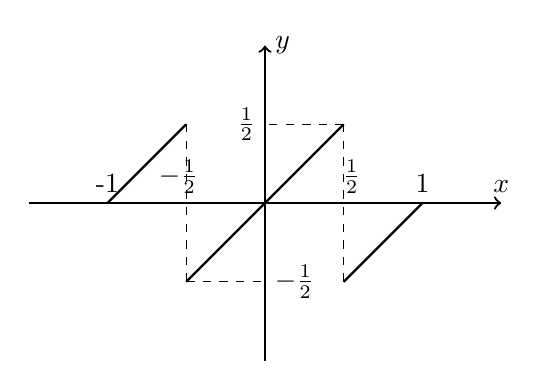
\begin{tikzpicture}
\draw [thick, ->] (-3,0) -- (3,0) node[above] {$x$};
\draw [thick, ->] (0,-2) -- (0,2) node[right] {$y$};
\draw [thick,-] (-1,-1) -- (1,1) node[above] at(2,0) {1};
\draw [thick,-] (1,-1) -- (2,0) node[above] at(-2,0) {-1};
\draw [thick,-] (-2,0) -- (-1,1);
\draw [dashed] (1,-1) -- (1,1) node[above] at(1.1,0) {$\frac{1}{2}$};
\draw [dashed] (-1,-1) -- (-1,1) node[above] at(-1.1,0) {$-\frac{1}{2}$};
\draw [dashed] (-1,-1) -- (0,-1) node[right] at(0,-1) {$-\frac{1}{2}$};
\draw [dashed] (1,1) -- (0,1) node[left] at(0,1) {$\frac{1}{2}$};
\end{tikzpicture}
\end{center}
\caption{Function $y=\text{mod}(x+\frac{1}{2},1)-\frac{1}{2}$}
\end{figure}

In the real examples, we found that we didn't need to do the periodic correction for each pair of particles in the neighbourlists. In fact, most pairs of particles are very close originally, we can modify the \texttt{eneryg} function code.
\begin{verbatim}
function energy(Config, V)
    """
    Function to calculate the total potential energy.
    V(r) is the pair potential.
    """
    nlist_i, nlist_j = update_neighbourlist(Config)
    E = 0.0
    for k = 1:length(nlist_i)
        i, j = nlist_i[k], nlist_j[k];
        xi, xj = Config.X[i], Config.X[j];
        dx = xj - xi;
        r = norm2(dx);    
        if r > 0.5*min(L,H)          # min(L,H) is the length scale of the system
           dX = inv_bins * dx;                   # using equation (3.4a)
           dX = dX - floor(dX);                  # using equation (3.4b)
           dX = dX - (dX > 0.5);                 # using equation (3.2)
           dx = bins * dX;                       # using equation (3.5)
           r = norm2(dx);
        end
        E = E + V(r);
    end
    return 0.5*E;
end
\end{verbatim}

This is much faster than the original code, and also faster than my own Matlab code. We compute the potential energy of one given granular system (with 1024 particles) for 1000 times using this modified code and the original code and my own Matlab code, the time costed are 0.32s, 2.14s and 0.87s respectively.

\end{document}